\begin{frame}{DISTILLED-SINGLE-SHOT-DETECTOR (DSSD)}
    {\bfseries{\scriptsize{(Steps 5 e 6)}}}
    \begin{figure}
        \centering
        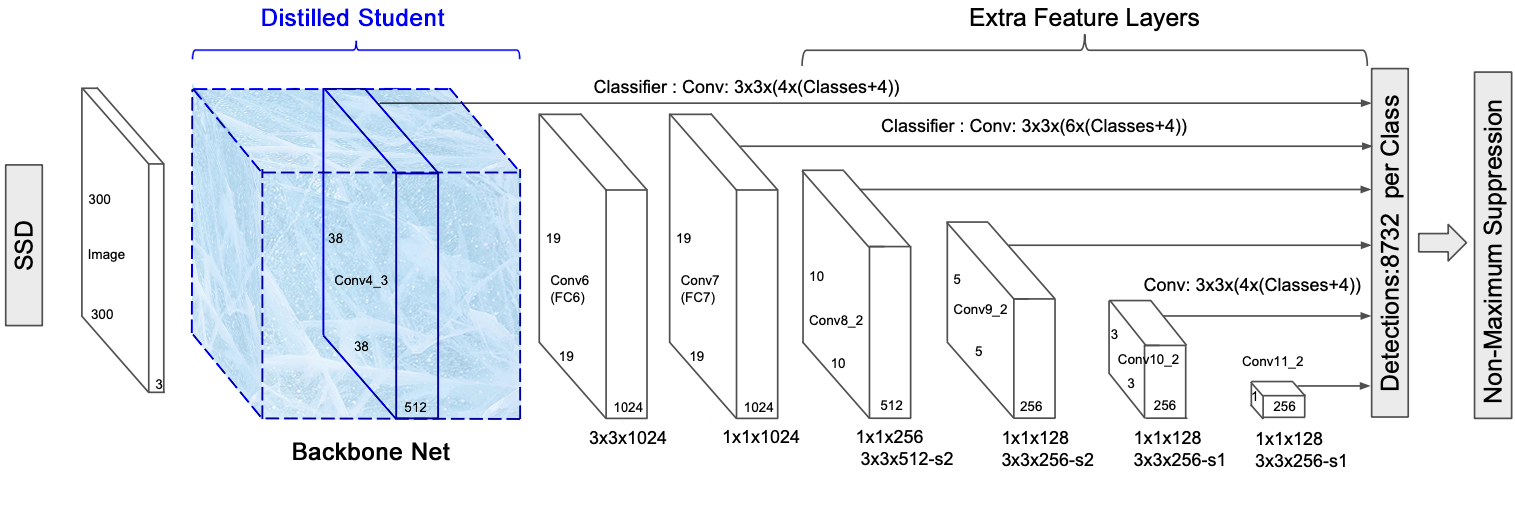
\includegraphics[width = \linewidth]{SSD_architecture_freeze.png}
        \centering
    \end{figure}
    \begin{minipage}{\linewidth}
        \centering
        \begin{minipage}{0.45\linewidth}
            \begin{block}{\centering 5. \emph{Integrazione}}
                Studente distillato come rete "{\bfseries{\emph{backbone}}}" nell'architettura {Single-Shot-Detector (SSD)}.    
            \end{block}
        \end{minipage}
        \hspace{0.5cm}
        \begin{minipage}{0.45\linewidth}
            \begin{block}{\centering 6. \emph{Fine Tuning}}
                Training del modello proposto \emph{DSSD} con {\bfseries{\emph{"congelamento"}}} \emph{(Freezing)} della rete \emph{backbone}.
            \end{block}
        \end{minipage}
    \end{minipage}   
\end{frame}

